% This template is borrowed from the Reed College LaTeX thesis template. Most of the work
% for the document class was done by Sam Noble (SN), as well as this
% template. Later comments etc. by Ben Salzberg (BTS). Additional
% restructuring and APA support by Jess Youngberg (JY).
% Your comments and suggestions are more than welcome; please email
% them to cus@reed.edu
%
% See http://web.reed.edu/cis/help/latex.html for help. There are a
% great bunch of help pages there, with notes on
% getting started, bibtex, etc. Go there and read it if you're not
% already familiar with LaTeX.
%
% Any line that starts with a percent symbol is a comment.
% They won't show up in the document, and are useful for notes
% to yourself and explaining commands.
% Commenting also removes a line from the document;
% very handy for troubleshooting problems. -BTS

% As far as I know, this follows the requirements laid out in
% the 2002-2003 Senior Handbook. Ask a librarian to check the
% document before binding. -SN

%%
%% Preamble
%%
% \documentclass{<something>} must begin each LaTeX document
\documentclass[12pt,twoside]{deuthesis}
% Packages are extensions to the basic LaTeX functions. Whatever you
% want to typeset, there is probably a package out there for it.
% Chemistry (chemtex), screenplays, you name it.
% Check out CTAN to see: http://www.ctan.org/
%%
\usepackage{graphicx,latexsym}
\usepackage{amsmath}
\usepackage{amssymb,amsthm}
\usepackage{longtable,booktabs,setspace}
\usepackage{chemarr} %% Useful for one reaction arrow, useless if you're not a chem major
\usepackage[hyphens]{url}
% Added by CII
\usepackage{hyperref}
\usepackage{lmodern}
\usepackage{float}
\floatplacement{figure}{H}
% End of CII addition
\usepackage{rotating}

% Next line commented out by CII
%%% \usepackage{natbib}
% Comment out the natbib line above and uncomment the following two lines to use the new
% biblatex-chicago style, for Chicago A. Also make some changes at the end where the
% bibliography is included.
%\usepackage{biblatex-chicago}
%\bibliography{thesis}


% Added by CII (Thanks, Hadley!)
% Use ref for internal links
\renewcommand{\hyperref}[2][???]{\autoref{#1}}
\def\chapterautorefname{Chapter}
\def\sectionautorefname{Section}
\def\subsectionautorefname{Subsection}
% End of CII addition

% Added by CII
\usepackage{caption}
\captionsetup{width=5in}
% End of CII addition

% \usepackage{times} % other fonts are available like times, bookman, charter, palatino

% Syntax highlighting #22

% To pass between YAML and LaTeX the dollar signs are added by CII
\title{Değişim Noktası Belirleme Yöntemleri ve Uygulamaları}
%\author{Pelin PEKERMerve AKEdanur Binnaz DURSUNAhmet ÇALI} %Tek yazar için
\author{Pelin PEKER \\ Merve AK \\ Edanur Binnaz DURSUN \\ Ahmet ÇALI} %Çok yazar için
% The month and year that you submit your FINAL draft TO THE LIBRARY (May or December)
\date{May 2024}
\division{İSTATİSTİK BÖLÜMÜ}
\advisor{Dr.~Engin YILDIZTEPE}
\institution{FEN FAKÜLTESİ}
\degree{Bitirme Projesi Raporu}
%If you have two advisors for some reason, you can use the following
% Uncommented out by CII
% End of CII addition

%%% Remember to use the correct department!
\department{İstatistik Bölümü}
% if you're writing a thesis in an interdisciplinary major,
% uncomment the line below and change the text as appropriate.
% check the Senior Handbook if unsure.
%\thedivisionof{The Established Interdisciplinary Committee for}
% if you want the approval page to say "Approved for the Committee",
% uncomment the next line
%\approvedforthe{Committee}

% Added by CII
%%% Copied from knitr
%% maxwidth is the original width if it's less than linewidth
%% otherwise use linewidth (to make sure the graphics do not exceed the margin)
\makeatletter
\def\maxwidth{ %
  \ifdim\Gin@nat@width>\linewidth
    \linewidth
  \else
    \Gin@nat@width
  \fi
}
\makeatother

\renewcommand{\contentsname}{Table of Contents}
% End of CII addition

\setlength{\parskip}{0pt}

% Added by CII

\providecommand{\tightlist}{%
  \setlength{\itemsep}{0pt}\setlength{\parskip}{0pt}}

\Acknowledgements{
Tüm çalışma süresince yönlendiriciliği, katkıları ve yardımları ile yanımızda olan danışmanımız Dr.~Engin YILDIZTEPE 'ye ve böyle bir çalışmayı yapmamız için bize fırsat tanıyan Dokuz Eylül Üniversitesi Fen Fakültesi İstatistik Bölümüne teşekkür ederiz.\\
\strut \\
\strut \\
Pelin PEKER\\
Merve AK\\
Edanur Binnaz DURSUN\\
Ahmet ÇALI\\
}

\Dedication{

}

\Preface{
``Değişim Noktası Belirleme Yöntemleri ve Uygulamaları'' başlıklı bitirme projesi raporu tarafıgitmdan okunmuş, kapsamı ve niteliği açısından bir Bitirme Projesi raporu olarak kabul edilmiştir.\\
\strut \\
\strut \\
Dr.~Engin YILDIZTEPE
}

\AbstractTR{
Değişim noktası verilerde meydana gelen beklenmedik anlamlı değişiklikler olarak tanımlanabilir. Değişim noktası tespit yöntemleri bu noktaları istatistiksel tekniklerle bulmayı amaçlar. Değişim noktası analizi finans, kalite kontrol, ağ analizi gibi çok farklı alanlarda kullanılmaktadır. Bu çalışmada değişim noktası tespit yöntemleri incelenmiştir. Çalışma kapsamında AMOC, BinSeg, parçalı regresyon, PELT ve Prophet algoritmaları kullanılmıştır. Algoritmaların uygulamadaki performanslarını belirlemek amacıyla yirmi yapay ve on bir gerçek veri kullanılmıştır. Performanslar F1 puanı ve kapsama ölçütü kullanılarak değerlendirilmiştir. F1 puanına göre en başarılı sonuçlar yapay verilerde BinSeg ile, gerçek verilerde parçalı regresyon ile alınmıştır. Kapsama ölçütüne göre ise yapay verilerde BinSeg ve parçalı regresyon, gerçek verilerde parçalı regresyon ile en iyi sonuçlar elde edilmiştir. Değişim noktası içeren yapay veri üretmek ve bahsedilen algoritmaları uygulayabilmek amacıyla bir RShiny web uygulaması geliştirilmiştir. Çalışmada R ve Python programlama dilleri kullanılmıştır.\\
\strut \\

\textbf{Anahtar Kelimeler:} Değişim noktası, AMOC, BinSeg, PELT, Prophet, Parçalı Regresyon, R shiny
}

\Abstract{
Change points can be defined as unexpected significant changes occurring in data. Change point detection methods aim to identify these points using statistical techniques. Change point analysis is utilized in various fields such as finance, quality control, and network analysis. In this study, change point detection methods were examined. AMOC, BinSeg, Segmented Regression, PELT, and Prophet algorithms were used within the scope of the study. To determine the performance of the algorithms in application, twenty artificial and eleven real datasets were employed. Performance was evaluated using the F1 score and cover metric. According to the F1 score, the most successful results were obtained with BinSeg on artificial data and with Segmented Regression on real data. Regarding the cover metric, BinSeg and Segmented Regression yielded the best results on artificial data, while Segmented Regression performed the best on real data. To generate artificial data containing change points and apply the mentioned algorithms, an R Shiny web application was developed. Both R and Python programming languages were used in the study.\\
\strut \\

\textbf{Keywords:} Changepoint, AMOC, BinSeg, Pelt, Prophet, Segmented Regression, R Shiny
}


% End of CII addition
%%
%% End Preamble
%%
%

\begin{document}

% Everything below added by CII
  \maketitle

\frontmatter % this stuff will be roman-numbered
\pagestyle{empty} % this removes page numbers from the frontmatter

\begin{preface}
	``Değişim Noktası Belirleme Yöntemleri ve Uygulamaları'' başlıklı bitirme projesi raporu tarafıgitmdan okunmuş, kapsamı ve niteliği açısından bir Bitirme Projesi raporu olarak kabul edilmiştir.\\
\strut \\
\strut \\
Dr.~Engin YILDIZTEPE
\end{preface}

  \begin{acknowledgements}
    Tüm çalışma süresince yönlendiriciliği, katkıları ve yardımları ile yanımızda olan danışmanımız Dr.~Engin YILDIZTEPE 'ye ve böyle bir çalışmayı yapmamız için bize fırsat tanıyan Dokuz Eylül Üniversitesi Fen Fakültesi İstatistik Bölümüne teşekkür ederiz.\\
    \strut \\
    \strut \\
    Pelin PEKER\\
    Merve AK\\
    Edanur Binnaz DURSUN\\
    Ahmet ÇALI\\
  \end{acknowledgements}

\begin{abstractTR}
	Değişim noktası verilerde meydana gelen beklenmedik anlamlı değişiklikler olarak tanımlanabilir. Değişim noktası tespit yöntemleri bu noktaları istatistiksel tekniklerle bulmayı amaçlar. Değişim noktası analizi finans, kalite kontrol, ağ analizi gibi çok farklı alanlarda kullanılmaktadır. Bu çalışmada değişim noktası tespit yöntemleri incelenmiştir. Çalışma kapsamında AMOC, BinSeg, parçalı regresyon, PELT ve Prophet algoritmaları kullanılmıştır. Algoritmaların uygulamadaki performanslarını belirlemek amacıyla yirmi yapay ve on bir gerçek veri kullanılmıştır. Performanslar F1 puanı ve kapsama ölçütü kullanılarak değerlendirilmiştir. F1 puanına göre en başarılı sonuçlar yapay verilerde BinSeg ile, gerçek verilerde parçalı regresyon ile alınmıştır. Kapsama ölçütüne göre ise yapay verilerde BinSeg ve parçalı regresyon, gerçek verilerde parçalı regresyon ile en iyi sonuçlar elde edilmiştir. Değişim noktası içeren yapay veri üretmek ve bahsedilen algoritmaları uygulayabilmek amacıyla bir RShiny web uygulaması geliştirilmiştir. Çalışmada R ve Python programlama dilleri kullanılmıştır.\\
\strut \\

\textbf{Anahtar Kelimeler:} Değişim noktası, AMOC, BinSeg, PELT, Prophet, Parçalı Regresyon, R shiny
\end{abstractTR}

\begin{abstract}
	Change points can be defined as unexpected significant changes occurring in data. Change point detection methods aim to identify these points using statistical techniques. Change point analysis is utilized in various fields such as finance, quality control, and network analysis. In this study, change point detection methods were examined. AMOC, BinSeg, Segmented Regression, PELT, and Prophet algorithms were used within the scope of the study. To determine the performance of the algorithms in application, twenty artificial and eleven real datasets were employed. Performance was evaluated using the F1 score and cover metric. According to the F1 score, the most successful results were obtained with BinSeg on artificial data and with Segmented Regression on real data. Regarding the cover metric, BinSeg and Segmented Regression yielded the best results on artificial data, while Segmented Regression performed the best on real data. To generate artificial data containing change points and apply the mentioned algorithms, an R Shiny web application was developed. Both R and Python programming languages were used in the study.\\
\strut \\

\textbf{Keywords:} Changepoint, AMOC, BinSeg, Pelt, Prophet, Segmented Regression, R Shiny
\end{abstract}


  \hypersetup{linkcolor=black}
  \setcounter{tocdepth}{2}
  \tableofcontents

  \listoftables

  \listoffigures


% This was added by EY
\newlength{\cslhangindent}
\setlength{\cslhangindent}{1.5em}
\newenvironment{CSLReferences}%
  {}%
  {\par}
\newenvironment{cslreferences}%
  {}%
  {\par}

\mainmatter % here the regular arabic numbering starts
\pagestyle{fancyplain} % turns page numbering back on

\hypertarget{thesisdownthesis_gitbook-default}{%
\chapter{thesisdown::thesis\_gitbook: default}\label{thesisdownthesis_gitbook-default}}

Placeholder

\hypertarget{Bolum2}{%
\chapter{Değişim Noktası}\label{Bolum2}}

Placeholder

\hypertarget{tek-deux11fiux15fim-noktasux131-tespiti}{%
\section{Tek Değişim Noktası Tespiti}\label{tek-deux11fiux15fim-noktasux131-tespiti}}

\hypertarget{birden-fazla-deux11fiux15fim-noktasux131-tespiti}{%
\section{Birden Fazla Değişim Noktası Tespiti}\label{birden-fazla-deux11fiux15fim-noktasux131-tespiti}}

\hypertarget{ikili-segmentasyon-algoritmasux131}{%
\subsection{İkili Segmentasyon Algoritması}\label{ikili-segmentasyon-algoritmasux131}}

\hypertarget{prophet}{%
\subsection{PROPHET}\label{prophet}}

\hypertarget{peltpruned-exact-linear-time}{%
\subsection{PELT(Pruned Exact Linear Time)}\label{peltpruned-exact-linear-time}}

\hypertarget{optimal-buxf6luxfctleme}{%
\subsubsection{Optimal Bölütleme}\label{optimal-buxf6luxfctleme}}

\hypertarget{pelt-yuxf6ntemi}{%
\subsubsection{PELT Yöntemi}\label{pelt-yuxf6ntemi}}

\hypertarget{paruxe7alux131-regresyon}{%
\subsection{Parçalı Regresyon}\label{paruxe7alux131-regresyon}}

\hypertarget{kapsama-uxf6luxe7uxfctuxfc}{%
\section{Kapsama Ölçütü}\label{kapsama-uxf6luxe7uxfctuxfc}}

\hypertarget{f1-puanux131}{%
\section{F1 Puanı}\label{f1-puanux131}}

\hypertarget{doux11fruluk-accuracy}{%
\subsubsection{Doğruluk (Accuracy)}\label{doux11fruluk-accuracy}}

\hypertarget{duyarlux131lux131k-recall}{%
\subsubsection{Duyarlılık (Recall)}\label{duyarlux131lux131k-recall}}

\hypertarget{kesinlik-precision}{%
\subsubsection{Kesinlik (Precision)}\label{kesinlik-precision}}

\hypertarget{f1-skoru-f1-score}{%
\subsubsection{F1 Skoru (F1 Score)}\label{f1-skoru-f1-score}}

\hypertarget{Bolum3}{%
\chapter{Uygulama}\label{Bolum3}}

Uygulamada yirmi yapay veri ve onbir gerçek veri kullanılmıştır. Yapay verilerin her biri farklı sayıda değişim noktasına sahip olacak şekilde üretilmiştir. Gerçek veriler ise farklı alanlardan alınmıştır. Verilerin performanslarını belirlemek amacıyla F1 puanı ve kapsama ölçütü kullanılmıştır. Çalışmada R ve Python programlama dilleri kullanılmıştır. Uygulamada kullanılan veriler ve kodlar github sayfasında (\url{https://github.com/eyildiztepe/ChangePointDetection}) paylaşılmıştır.

\hypertarget{veri}{%
\section{Veri}\label{veri}}

Bu bölümde üretilen yapay veriler ve uygulamada kullanılan gerçek veriler hakkında bilgi verilmiştir.

\hypertarget{yapay-veri}{%
\subsection{Yapay Veri}\label{yapay-veri}}

Çalışmada kullanılan yapay veriler farklı sayıda değişim noktasına (DN) sahip olacak şekilde R programlama dili kullanılarak üretilmiştir. Yapay verilerin örneklem genişlikleri, ortalaması 2000, standart sapması 500 olan Normal dağılımndan, verideki değişim noktası sayısı ortalaması 2.8 olan Poisson dağılımından ve DN'lerin konumları ise Uniform dağılımından üretilmiştir. Kullanılan verilerin özellikleri Tablo \ref{tab:nvar1}'de verilmiştir.

\begin{longtable}[]{@{}llll@{}}
\caption{\label{tab:nvar1} Yapay Veriler}\tabularnewline
\toprule\noalign{}
Veri & Gözlem Sayısı & DN Sayısı & DN Konumu \\
\midrule\noalign{}
\endfirsthead
\toprule\noalign{}
Veri & Gözlem Sayısı & DN Sayısı & DN Konumu \\
\midrule\noalign{}
\endhead
\bottomrule\noalign{}
\endlastfoot
1 & 1687 & 4 & 516, 578 ,779,1499 \\
2 & 2092 & 3 & 564,1003,1347 \\
3 & 1582 & 4 & 175,553,1186,1347 \\
4 & 2798 & 3 & 951,985,2315 \\
5 & 2165 & 3 & 1034,1835,1892 \\
6 & 1590 & 4 & 631,698,1208,1481 \\
7 & 2244 & 1 & 1578 \\
8 & 2369 & 3 & 788,958,1768 \\
9 & 2288 & 4 & 316,493, 587,1606 \\
10 & 1847 & 4 & 153,300, 469,1172 \\
11 & 2756 & 3 & 2119,2168,2377 \\
12 & 2195 & 5 & 909,1004,1317,1422,1749 \\
13 & 1689 & 2 & 479,611 \\
14 & 893 & 2 & 552,837 \\
15 & 2562 & 1 & 575 \\
16 & 1978 & 1 & 293 \\
17 & 1992 & 2 & 955,1798 \\
18 & 2472 & 3 & 1470,1786,2365 \\
19 & 2411 & 3 & 393,874,1047 \\
20 & 2297 & 2 & 79,1622 \\
\end{longtable}

\hypertarget{geruxe7ek-veri}{%
\subsection{Gerçek Veri}\label{geruxe7ek-veri}}

Çalışmada farklı alanlardan gerçek veriler kullanılmıştır. Veriler (\url{https://github.com/alan-turing-institute/TCPD/tree/master/datasets}) adresinden temin edilmiştir. Gerçek verilerin özellikleri Tablo \ref{tab:ngercek}'de verilmiştir.

\begin{longtable}[]{@{}lllllll@{}}
\caption{\label{tab:ngercek} Gerçek Veriler}\tabularnewline
\toprule\noalign{}
Veri & GS & 1.DNS & 2.DNS & 3.DNS & 4.DNS & 5.DNS \\
\midrule\noalign{}
\endfirsthead
\toprule\noalign{}
Veri & GS & 1.DNS & 2.DNS & 3.DNS & 4.DNS & 5.DNS \\
\midrule\noalign{}
\endhead
\bottomrule\noalign{}
\endlastfoot
Bitcoin & NA & 4 & 1 & 1 & 7 & 7 \\
Brent-spot. & 500 & 3 & 2 & 5 & 9 & 11 \\
Children-per women & 301 & 2 & 1 & 2 & 4 & 2 \\
Co2- canada & 215 & 2 & 6 & 2 & 5 & 7 \\
Debt -Ireland & 21 & 2 & 2 & 2 & 4 & 2 \\
Rail-lines & 37 & 2 & 2 & 2 & 2 & 1 \\
Rather-stock & 600 & 1 & 2 & 1 & 2 & 2 \\
Scanline-42049 & 481 & 10 & 7 & 2 & 7 & 7 \\
Shangai-license & 205 & 1 & 1 & 1 & 1 & 2 \\
Usd-isk & 247 & 2 & 4 & 1 & 3 & 2 \\
Well-log & 675 & 11 & 9 & 9 & 2 & 17 \\
\end{longtable}

\emph{GS: Gözlem sayısı ,DNS: Değişim Noktası Sayısı}

Çalışmada kullanılan gerçek veriler 5 ayrı işaretleyici tarafından işaretlenmiştir (Van den Burg ve Williams, 2020).Bu nedenle değişim noktası konumları değişiklik göstermektedir .

\hypertarget{deux11fiux15fim-noktasux131-analizi}{%
\section{Değişim Noktası Analizi}\label{deux11fiux15fim-noktasux131-analizi}}

Bu bölümde kullanılan yöntemler ile elde edilen sonuçlara yer verilmiştir. Kullanılan fonksiyonların varsayılan ayarları ile elde edilen sonuçlar F1 puanı varsayılan ve kapsama ölçütü varsayılan olarak adlandırılmıştır. Ayrıca, argümanların değerleri değiştirilerek elde edilen en iyi sonuçlar F1 puanı ayarlanmış ve kapsama ölçütü ayarlanmış olarak sunulmuştur.

\hypertarget{yapay-veriler-iuxe7in-sonuuxe7lar}{%
\subsection{Yapay Veriler için Sonuçlar}\label{yapay-veriler-iuxe7in-sonuuxe7lar}}

Bu bölümde yapay veriler için elde edilen sonuçlara yer verilmiştir.

\begin{longtable}[]{@{}llllll@{}}
\caption{\label{tab:nvar8} F1 puanı (Varsayılan)}\tabularnewline
\toprule\noalign{}
Veri & AMOC & BINSEG & SEGMENTED & PROPHET & PELT \\
\midrule\noalign{}
\endfirsthead
\toprule\noalign{}
Veri & AMOC & BINSEG & SEGMENTED & PROPHET & PELT \\
\midrule\noalign{}
\endhead
\bottomrule\noalign{}
\endlastfoot
1 & 0,5714 & 0,9091 & 0,2857 & 0,2857 & 0,4000 \\
2 & 0,6667 & 0,4000 & 0,3333 & 0,1818 & 0,4444 \\
3 & 0,5714 & 0,9091 & 0,1290 & 0,2000 & 0,4000 \\
4 & 0,6667 & 0,8000 & 0,3333 & 0,2222 & 0,7500 \\
5 & 0,6667 & 0,6000 & 0,4444 & 0,2500 & 0,6666 \\
6 & 0,5714 & 0,5455 & 0,4000 & 0,1538 & 0,4000 \\
7 & 0,5000 & 0,2500 & 0,5000 & 0,3333 & 0,5000 \\
8 & 0,6667 & 0,8000 & 0,5000 & 0,2222 & 0,6000 \\
9 & 0,2857 & 0,5455 & 0,4000 & 0,1818 & 0,3636 \\
10 & 0,5714 & 0,7273 & 0,6000 & 0,1666 & 0,4615 \\
11 & 0,6667 & 0,6000 & 0,5000 & 0,2222 & 0,4444 \\
12 & 0,5000 & 0,8333 & 0,1666 & 0,1666 & 0,5000 \\
13 & 0,8000 & 0,6667 & 0,6666 & 0,2857 & 0,5714 \\
14 & 0,8000 & 0,6667 & 0,6666 & 0,2857 & 0,5714 \\
15 & 0,9998 & 0,5000 & 0,5000 & 0,4000 & 0,4000 \\
16 & 0,9999 & 0,5000 & 0,5000 & 0,4000 & 0,4000 \\
17 & 0,8000 & 0,6667 & 0,6666 & 0,2857 & 0,5714 \\
18 & 0,6667 & 0,8000 & 0,5000 & 0,2222 & 0,4000 \\
19 & 0,6667 & 0,8000 & 0,5000 & 0,2222 & 0,4444 \\
20 & 0,8000 & 0,4444 & 0,3333 & 0,2857 & 0,2857 \\
\end{longtable}

Algoritmalar varsayılan parametre ayarlarıyla çalıştırıldığında (\ref{tab:nvar8}), yirmi yapay verinin sekizinde BinSeg, altısında AMOC ve birinde PELT 0,7 ve üzerinde F1 puanına sahipken, parçalı regresyon ve Prophet algoritmasında F1 puanı 0,7 ve üzerinde olan veri bulunmamaktadır.
Varsayılan parametrelerle çalıştırılan algoritmalardan Prophet on yedi, parçalı regresyon üç, AMOC, BinSeg ve Pelt algoritmalarında birer tane 0,3'ün altında F1 puanına sahip veri bulunmaktadır.

\begin{longtable}[]{@{}llllll@{}}
\caption{\label{tab:nvar9} Kapsama Ölçütü (Varsayılan)}\tabularnewline
\toprule\noalign{}
Veri & AMOC & BINSEG & SEGMENTED & PROPHET & PELT \\
\midrule\noalign{}
\endfirsthead
\toprule\noalign{}
Veri & AMOC & BINSEG & SEGMENTED & PROPHET & PELT \\
\midrule\noalign{}
\endhead
\bottomrule\noalign{}
\endlastfoot
1 & 0,5975 & 0,9895 & 0,3740 & 0,3607 & 0,6843 \\
2 & 0,5388 & 0,8881 & 0,5185 & 0,5600 & 0,7686 \\
3 & 0,4937 & 0,9943 & 0,2397 & 0,5151 & 0,7953 \\
4 & 0,5850 & 0,8989 & 0,4876 & 0,5495 & 0,8897 \\
5 & 0,7707 & 0,9687 & 0,8126 & 0,6164 & 0,7706 \\
6 & 0,6079 & 0,8822 & 0,7007 & 0,3625 & 0,5339 \\
7 & 0,9648 & 0,7995 & 0,7807 & 0,4670 & 0,8523 \\
8 & 0,6084 & 0,8848 & 0,6725 & 0,6173 & 0,7047 \\
9 & 0,6629 & 0,9467 & 0,4937 & 0,5129 & 0,6060 \\
10 & 0,6269 & 0,9288 & 0,7368 & 0,4726 & 0,4510 \\
11 & 0,8764 & 0,9464 & 0,8185 & 0,9991 & 0,6856 \\
12 & 0,5639 & 0,8220 & 0,6032 & 0,6158 & 0,5461 \\
13 & 0,8771 & 0,7478 & 0,8771 & 0,5563 & 0,4660 \\
14 & 0,8932 & 0,9567 & 0,8911 & 0,4304 & 0,7085 \\
15 & 0,9992 & 0,9863 & 0,8634 & 0,5091 & 0,4972 \\
16 & 0,9950 & 0,7715 & 0,8828 & 0,4541 & 0,4058 \\
17 & 0,8408 & 0,8620 & 0,8403 & 0,5809 & 0,5871 \\
18 & 0,7744 & 0,9956 & 0,8502 & 0,4184 & 0,4871 \\
19 & 0,6932 & 0,9925 & 0,7623 & 0,4422 & 0,4285 \\
20 & 0,5905 & 0,7208 & 0,4578 & 0,4711 & 0,5644 \\
\end{longtable}

Tablo \ref{tab:nvar9}'daki sonuçlara göre, BinSeg varsayılan parametre ayarlarıyla çalıştırıldığında tüm verilerde 0,7'nin üzerinde kapsama ölçütü değerine sahiptir. Parçalı regresyon on ikisinde, AMOC dokuzunda, Pelt yedisinde ve Prophet birinde 0,7 ve üzerinde kapsama ölçütü değerine sahip olduğu görülmektedir.

Varsayılan ayarlar çalıştırılan algoritmalardan sadece parçalı regresyonda bir veri 0,3'ün altında kapsama ölçütü değerine sahiptir.

\begin{longtable}[]{@{}llllll@{}}
\caption{\label{tab:nvar10} F1 Puanı (Ayarlanmış)}\tabularnewline
\toprule\noalign{}
Veri & AMOC & BINSEG & SEGMENTED & PROPHET & PELT \\
\midrule\noalign{}
\endfirsthead
\toprule\noalign{}
Veri & AMOC & BINSEG & SEGMENTED & PROPHET & PELT \\
\midrule\noalign{}
\endhead
\bottomrule\noalign{}
\endlastfoot
1 & 0,5714 & 0,9997 & 0,4444 & 0,2500 & 0,6000 \\
2 & 0,6667 & 0,5000 & 0,5000 & 0,4000 & 0,5000 \\
3 & 0,5714 & 0,9994 & 0,4000 & 0,2500 & 0,4000 \\
4 & 0,6667 & 0,9996 & 0,4000 & 0,2500 & 0,7500 \\
5 & 0,6667 & 0,7500 & 0,4000 & 0,2857 & 0,6666 \\
6 & 0,5714 & 0,6000 & 0,4000 & 0,3333 & 0,2857 \\
7 & 0,5000 & 0,5000 & 0,5000 & 0,4000 & 0,5000 \\
8 & 0,6667 & 0,7500 & 0,5000 & 0,2500 & 0,5454 \\
9 & 0,2857 & 0,6000 & 0,4000 & 0,2222 & 0,3636 \\
10 & 0,5714 & 0,8000 & 0,6000 & 0,2000 & 0,6000 \\
11 & 0,6667 & 0,7500 & 0,5000 & 0,2500 & 0,5714 \\
12 & 0,5000 & 0,8333 & 0,1666 & 0,3636 & 0,5000 \\
13 & 0,8000 & 0,9987 & 0,6666 & 0,3333 & 0,6666 \\
14 & 0,8000 & 0,6667 & 0,6666 & 0,3333 & 0,6666 \\
15 & 0,9998 & 0,9989 & 0,5000 & 0,5000 & 0,5000 \\
16 & 0,9999 & 0,9967 & 0,5000 & 0,5000 & 0,5000 \\
17 & 0,8000 & 0,9985 & 0,6666 & 0,3333 & 0,6666 \\
18 & 0,6667 & 0,9978 & 0,5000 & 0,2500 & 0,5000 \\
19 & 0,6667 & 0,9949 & 0,5000 & 0,2500 & 0,5000 \\
20 & 0,8000 & 0,6667 & 0,3333 & 0,3333 & 0,3333 \\
\end{longtable}

Ayarlanmış parametreler sonucunda en iyi F1 puanı değerleri BinSeg ile elde edilmiştir. Prophet ve parçalı regresyon algoritmalarında hiç bir veri 0,7 ve üzerinde F1 puanına sahip değildir. Pelt algoritmasında bir tane verinin 0,7'nin üzerinde olduğu görülmektedir.

Prophet algoritmasının en kötü F1 puanı değerlerini verdiği görülmektedir. AMOC, parçalı regresyon ve Pelt algoritmalarında 0,3 'ün altında birer tane veri bulunmaktadır.

\begin{longtable}[]{@{}llllll@{}}
\caption{\label{tab:nvar11} Kapsama Ölçütü (Ayarlanmış)}\tabularnewline
\toprule\noalign{}
Veri & AMOC & BINSEG & SEGMENTED & PROPHET & PELT \\
\midrule\noalign{}
\endfirsthead
\toprule\noalign{}
Veri & AMOC & BINSEG & SEGMENTED & PROPHET & PELT \\
\midrule\noalign{}
\endhead
\bottomrule\noalign{}
\endlastfoot
1 & 0,5975 & 0,9930 & 0,9930 & 0,6104 & 0,7081 \\
2 & 0,5388 & 0,8914 & 0,8914 & 0,6793 & 0,8194 \\
3 & 0,4937 & 0,9950 & 0,9950 & 0,6152 & 0,9246 \\
4 & 0,5850 & 0,9957 & 0,9957 & 0,6830 & 0,8840 \\
5 & 0,7707 & 0,9688 & 0,9688 & 0,7494 & 0,7706 \\
6 & 0,6079 & 0,8853 & 0,8853 & 0,3967 & 0,5599 \\
7 & 0,9648 & 0,9648 & 0,9648 & 0,6002 & 0,9670 \\
8 & 0,6084 & 0,8831 & 0,8831 & 0,6700 & 0,7364 \\
9 & 0,6629 & 0,9467 & 0,9467 & 0,5665 & 0,6067 \\
10 & 0,6269 & 0,9092 & 0,9092 & 0,4866 & 0,7201 \\
11 & 0,8764 & 0,9689 & 0,9689 & 0,9998 & 0,9387 \\
12 & 0,5639 & 0,8220 & 0,8220 & 0,6338 & 0,5604 \\
13 & 0,8771 & 0,9976 & 0,9976 & 0,6158 & 0,6509 \\
14 & 0,8932 & 0,9567 & 0,9567 & 0,5356 & 0,8589 \\
15 & 0,9992 & 0,9992 & 0,9992 & 0,5255 & 0,8189 \\
16 & 0,9950 & 0,9950 & 0,9950 & 0,5825 & 0,7296 \\
17 & 0,8408 & 0,9980 & 0,9980 & 0,7171 & 0,7905 \\
18 & 0,7744 & 0,9976 & 0,9976 & 0,4701 & 0,6171 \\
19 & 0,6932 & 0,9983 & 0,9983 & 0,4816 & 0,6680 \\
20 & 0,5905 & 0,9854 & 0,9854 & 0,5511 & 0,7184 \\
\end{longtable}

Ayarlanan parametreler ile hesaplanan kapsama ölçütü değerinin BinSeg ve parçalı regresyon algoritmalarının tamamında 0,8'in üzerinde olduğu görülmektedir. Pelt için on dört, AMOC için dokuz ve Prophet algortiması için üç verinin 0,7'nin üzerindekapsama ölçütü değerine sahip olduğu görülmektedir.
Ayarlanan parametrelerle çalıştırılan beş farklı algoritmanın kullanıldığı yirmi verinin hiçbirinde 0,3'ün altından kapsama ölçütü değeri bulunmamaktadır.

\hypertarget{yapay-veriler-iuxe7in-friedman-test}{%
\subsection{Yapay Veriler için Friedman Test}\label{yapay-veriler-iuxe7in-friedman-test}}

\begin{verbatim}
Loading required package: PMCMRplus
\end{verbatim}

\begin{verbatim}

    Friedman rank sum test

data:  sim
Friedman chi-squared = 54.674, df = 4, p-value = 3.803e-11
\end{verbatim}

\begin{align*}
& H_0: \text{Algoritmalar arasında istatistiksel olarak anlamlı bir fark yoktur.} \\
& H_1: \text{Algoritmalar arasında en az birinde istatistiksel olarak anlamlı bir fark vardır.}
\end{align*}

\(p\)-değeri 0.05 (\(\alpha\))'den küçüktür. Bu nedenle \(H_0\) hipotezi reddedilmiştir, algoritmalar arasında en az bir tanesi farklıdır.

\hypertarget{yapay-veriler-iuxe7in-nemenyi-test}{%
\subsubsection{Yapay Veriler için Nemenyi Test}\label{yapay-veriler-iuxe7in-nemenyi-test}}

\begin{verbatim}

    Pairwise comparisons using Nemenyi-Wilcoxon-Wilcox all-pairs test for a two-way balanced complete block design
\end{verbatim}

\begin{verbatim}
data: y
\end{verbatim}

\begin{verbatim}
            AMOC    BinSeg  Parçalı Reg Prophet
BinSeg      0.00074 -       -           -      
Parçalı Reg 0.00074 1.00000 -           -      
Prophet     0.49732 2.8e-07 2.8e-07     -      
PELT        0.99964 0.00166 0.00166     0.37348
\end{verbatim}

\begin{verbatim}

P value adjustment method: single-step
\end{verbatim}

\begin{itemize}
    \item AMOC ve BinSeg algoritmaları arasında istatistiksel olarak anlamlı fark vardır.
    \item Parçalı Regresyon ve AMOC algoritmaları arasında istatistiksel olarak anlamlı fark vardır.
    \item Prophet ile BinSeg ve Parçalı Regresyon algoritmaları arasında istatistiksel olarak anlamlı fark vardır.
    \item PELT ile BinSeg ve Parçalı Regresyon algoritmaları arasında istatistiksel olarak anlamlı fark vardır.
\end{itemize}

\hypertarget{geruxe7ek-veriler-iuxe7in-sonuuxe7lar}{%
\subsection{Gerçek Veriler için Sonuçlar}\label{geruxe7ek-veriler-iuxe7in-sonuuxe7lar}}

Bu bölümde gerçek veriler için elde edilen sonuçlara yer verilmiştir.

\begin{longtable}[]{@{}llllll@{}}
\caption{\label{tab:nvar2} F1 puanı (Varsayılan)}\tabularnewline
\toprule\noalign{}
Veri & AMOC & BINSEG & PELT & SEGMENTED & PROPHET \\
\midrule\noalign{}
\endfirsthead
\toprule\noalign{}
Veri & AMOC & BINSEG & PELT & SEGMENTED & PROPHET \\
\midrule\noalign{}
\endhead
\bottomrule\noalign{}
\endlastfoot
Bitcoin & 0,3670 & 0,4897 & 0,2663 & 0,3670 & 0,2341 \\
Brent-spot & 0,2718 & 0,6431 & 0,4244 & 0,6590 & 0,3904 \\
Children-per women & 0,6175 & 0,5902 & 0,3366 & 0,8440 & 0,5168 \\
Co2- canada & 0,5441 & 0,8194 & 0,8194 & 0,3938 & 0,6315 \\
Debt -Ireland & 0,7603 & 1,0000 & 0,7603 & 0,7603 & 0,6086 \\
Rail-lines & 0,8462 & 0,8000 & 0,4690 & 1,0000 & 0,2666 \\
Rather-stock & 0,2718 & 0,3392 & 0,4710 & 0,4886 & 0,5292 \\
Scanline-42049 & 0,4926 & 0,7400 & 0,5151 & 0,2463 & 0,3902 \\
Shangai-license & 0,8679 & 0,6511 & 0,6666 & 0,6495 & 0,5316 \\
Usd-isk & 0,7854 & 0,6093 & NA & 0,7881 & 0,5956 \\
Well-log & NA & 0,7289 & 0,4235 & 0,6912 & 0,3589 \\
\end{longtable}

Varsayılan parametre ayarlarıyla algoritmalar çalıştırıldığında, on bir verinin beşinde BinSeg, dördünde AMOC ve parçalı regresyon, ikisinde PELT 0,7 ve üzerinde F1 puanına sahipken Prophet algoritmasında F1 puanı 0,7 ve üzerinde olan veri bulunmamaktadır.

Varsayılan ayarlarda, on bir verinin ikisinde AMOC ve Prophet ile, birinde PELT ve parçalı regresyon ile 0,3'ün altında F1 puanı elde edilmiştir.

BinSeg algoritmasında F1 puanı 0,3 ve altında olan veri bulunmamaktadır.
Değişim noktası tespit edilemeyen durumlar (NA) ile gösterilmiştir.

\begin{longtable}[]{@{}llllll@{}}
\caption{\label{tab:nvar3} Kapsama Ölçütü (Varsayılan)}\tabularnewline
\toprule\noalign{}
Veri & AMOC & BINSEG & PELT & SEGMENTED & PROPHET \\
\midrule\noalign{}
\endfirsthead
\toprule\noalign{}
Veri & AMOC & BINSEG & PELT & SEGMENTED & PROPHET \\
\midrule\noalign{}
\endhead
\bottomrule\noalign{}
\endlastfoot
Bitcoin & 0,7640 & 0,7354 & 0,3022 & 0,5322 & 0,1941 \\
Brent-spot & 0,4251 & 0,5921 & 0,4535 & 0,4945 & 0,2992 \\
Children-per women & 0,7838 & 0,7663 & 0,7721 & 0,6282 & 0,2753 \\
Co2- canada & 0,5264 & 0,7291 & 0,7393 & 0,5135 & 0,3409 \\
Debt -Ireland & 0,5844 & 0,6607 & 0,5446 & 0,5861 & 0,4000 \\
Rail-lines & 0,7682 & 0,7732 & 0,4408 & 0,7890 & 0,3081 \\
Rather-stock & 0,3870 & 0,3923 & 0,3970 & 0,5164 & 0,3470 \\
Scanline-42049 & 0,4305 & 0,7502 & 0,4157 & 0,3859 & 0,3249 \\
Shangai-license & 0,9105 & 0,7691 & 0,3132 & 0,8272 & 0,2458 \\
Usd-isk & 0,8577 & NA & NA & 0,5248 & 0,2752 \\
Well-log & 0,4527 & 0,7696 & 0,4285 & 0,4146 & 0,3743 \\
\end{longtable}

Varsayılan ayarlar ile, on bir verinin yedisinde BinSeg, beşinde AMOC, ikisinde PELT ve parçalı regresyon ile 0,7 ve üzerinde kapsama ölçütü değerleri elde edilmiştir.

Prophet algoritmasında hiçbir veri için kapsama ölçütü değeri 0,7 nin üzerinde değildir.
Varsayılan ayarlar ile Prophet algoritmasında başarılı kapsama ölçütü değerleri elde edilemediği görülmektedir. Prophet on bir verinin beşinde 0,3 ve altında kapsama ölçütü değerine sahiptir.
Değişim noktası tespit edilemeyen durumlar (NA) ile gösterilmiştir.

\begin{longtable}[]{@{}llllll@{}}
\caption{\label{tab:nvar4} F1 Puanı (Ayarlanmış)}\tabularnewline
\toprule\noalign{}
Veri & AMOC & BINSEG & PELT & SEGMENTED & PROPHET \\
\midrule\noalign{}
\endfirsthead
\toprule\noalign{}
Veri & AMOC & BINSEG & PELT & SEGMENTED & PROPHET \\
\midrule\noalign{}
\endhead
\bottomrule\noalign{}
\endlastfoot
Bitcoin & 0,3670 & 0,6124 & 0,3940 & 0,4523 & 0,2743 \\
Brent-spot & 0,2718 & 0,6341 & 0,4481 & 0,6590 & 0,3704 \\
Children-per women & 0,6175 & 0,5902 & 0,6388 & 0,8440 & 0,5168 \\
Co2- canada & 0,5441 & 0,8776 & 0,3595 & 0,7142 & 0,6045 \\
Debt -Ireland & 0,7603 & 0,9583 & 0,9583 & 0,9795 & 0,9795 \\
Rail-lines & 0,8461 & 0,8316 & 0,7234 & 0,9655 & 0,9655 \\
Rather-stock & 0,2718 & 0,3728 & 0,5316 & 0,4243 & 0,5292 \\
Scanline-42049 & 0,4926 & 0,8331 & 0,5704 & 0,8648 & 0,4581 \\
Shangai-license & 0,8679 & 0,6511 & 0,2025 & 0,6495 & 0,5316 \\
Usd-isk & 0,7854 & 0,6093 & 0,6007 & 0,7881 & 0,5956 \\
Well-log & 0,2791 & 0,7289 & 0,5760 & 0,6912 & 0,3589 \\
\end{longtable}

Ayarlanmış parametreler ile en iyi F1 puanı değerleri parçalı regresyon ile alınmıştır. On bir veri setinin altısında parçalı regresyon, beşinde BinSeg, dördünde AMOC, ikisinde PELT ve Prophet'in 0,7 ve üzerinde F1 puanına sahip olduğu görülmektedir.

Tablo \ref{tab:nvar4}'e göre parçalı regresyon ve BinSeg algoritmaları denenen tüm gerçek veriler için 0,3 ve üzerinde F1 puanı elde etmişlerdir. Ancak AMOC algoritması için F1 puanı onbir verinin üçünde 0,3'ün altındadır.

\begin{longtable}[]{@{}llllll@{}}
\caption{\label{tab:nvar5} Kapsama Ölçütü (Ayarlanmış)}\tabularnewline
\toprule\noalign{}
Veri & AMOC & BINSEG & PELT & SEGMENTED & PROPHET \\
\midrule\noalign{}
\endfirsthead
\toprule\noalign{}
Veri & AMOC & BINSEG & PELT & SEGMENTED & PROPHET \\
\midrule\noalign{}
\endhead
\bottomrule\noalign{}
\endlastfoot
Bitcoin & 0,7640 & 0,4352 & 0,2182 & 0,3833 & 0,2045 \\
Brent-spot & 0,4251 & 0,4858 & 0,3257 & 0,5273 & 0,3206 \\
Children-per women & 0,7938 & 0,7625 & 0,7635 & 0,7062 & 0,3485 \\
Co2- canada & 0,5264 & 0,7001 & 0,7494 & 0,6622 & 0,4366 \\
Debt -Ireland & 0,5844 & 0,8136 & 0,7042 & 0,8217 & 0,6919 \\
Rail-lines & 0,7665 & 0,7731 & 0,5113 & 0,6964 & 0,6222 \\
Rather-stock & 0,3870 & 0,3941 & 0,4840 & 0,4488 & 0,3470 \\
Scanline-42049 & 0,4305 & 0,8570 & 0,4157 & 0,7944 & 0,4097 \\
Shangai-license & 0,9105 & 0,7961 & 0,3955 & 0,8058 & 0,3625 \\
Usd-isk & 0,8577 & 0,7549 & 0,5609 & 0,7819 & 0,4211 \\
Well-log & 0,4527 & 0,6371 & 0,4873 & 0,5511 & 0,4615 \\
\end{longtable}

Ayarlanmış parametreler ile algoritmalar çalıştırıldığında, kapsama ölçütüne göre en iyi sonuçları BinSeg algoritması vermiştir. Denenen on bir verinin yedisinde BinSeg, beşinde AMOC ve parçalı regresyon, üçünde PELT 0,7 ve üzerinde kapsama metriğine sahipken Prophet algoritmasında kapsama metriği 0,7 ve üzerinde olan veri bulunmamaktadır.

Çalışmada incelenen algoritmaların ihtiyaç duyduğu parametre değerleri verilere göre en uygun hale getirildiğinde BinSeg ve parçalı regresyon algoritmalarının diğerlerine göre değişim noktalarının konumlarını belirlemede daha başarılı olduğu görülmüştür.

\hypertarget{geruxe7ek-veriler-iuxe7in-friedman-test}{%
\subsection{Gerçek Veriler için Friedman Test}\label{geruxe7ek-veriler-iuxe7in-friedman-test}}

\begin{verbatim}

    Friedman rank sum test

data:  real
Friedman chi-squared = 19.564, df = 4, p-value = 0.0006088
\end{verbatim}

\begin{align*}
& H_0: \text{Algoritmalar arasında istatistiksel olarak anlamlı bir fark yoktur.} \\
& H_1: \text{Algoritmalar arasında en az birinde istatistiksel olarak anlamlı bir fark vardır.}
\end{align*}

\(p\)-değeri 0.05 (\(\alpha\))'den küçüktür. Bu nedenle \(H_0\) hipotezi reddedilmiştir, algoritmalar arasında en az bir tanesi farklıdır.

\hypertarget{geruxe7ek-veriler-iuxe7in-nemenyi-test}{%
\subsubsection{Gerçek Veriler için Nemenyi Test}\label{geruxe7ek-veriler-iuxe7in-nemenyi-test}}

\begin{verbatim}

    Pairwise comparisons using Nemenyi-Wilcoxon-Wilcox all-pairs test for a two-way balanced complete block design
\end{verbatim}

\begin{verbatim}
data: y
\end{verbatim}

\begin{verbatim}
            AMOC    BinSeg  PELT    Parçalı Reg
BinSeg      0.87972 -       -       -          
PELT        0.96200 0.48569 -       -          
Parçalı Reg 0.96200 0.99884 0.66078 -          
Prophet     0.02510 0.00088 0.14727 0.00252    
\end{verbatim}

\begin{verbatim}

P value adjustment method: single-step
\end{verbatim}

Prophet ile AMOC, BinSeg ve parçalı regresyon algoritmaları arasında istatistiksel olarak anlamlı bir fark vardır.

\hypertarget{kademeli-egzersiz-test-verileri}{%
\section{Kademeli Egzersiz Test Verileri}\label{kademeli-egzersiz-test-verileri}}

Bu bölümde 15 sporcunun kademeli bir rampa testi sonucunda elde edilen veriler kullanılarak eşik egzersiz şiddetlerini değişim noktası belirleme yöntemleri ile tespit etmek denenmiştir.

\begin{figure}
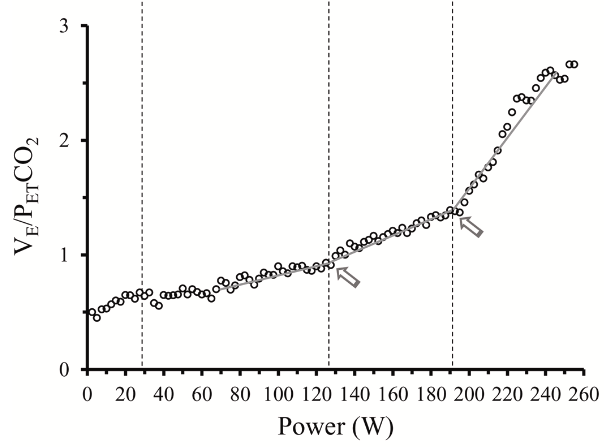
\includegraphics[width=302px,height=228px]{figure/vepetco2} \caption{Ve/PetCO2-Watt}\label{fig:unnamed-chunk-5}
\end{figure}

\begin{longtable}[]{@{}llll@{}}
\caption{\label{tab:nvar6} Kapsama Ölçütü (Ayarlanmış)}\tabularnewline
\toprule\noalign{}
Veri & BINSEG & SEGMENTED & PELT \\
\midrule\noalign{}
\endfirsthead
\toprule\noalign{}
Veri & BINSEG & SEGMENTED & PELT \\
\midrule\noalign{}
\endhead
\bottomrule\noalign{}
\endlastfoot
1 & 0,7023 & 0,6688 & 0,7340 \\
2 & NA & 0,8232 & NA \\
3 & NA & 0,5097 & NA \\
4 & 0,7485 & 0,9547 & 0,7308 \\
5 & 0,9326 & 0,8972 & 0,7314 \\
6 & NA & 0,7793 & NA \\
7 & NA & 0,9493 & NA \\
8 & 1,0000 & 0,8930 & 0,8425 \\
9 & 0,8181 & 0,9545 & 0,8723 \\
10 & 0,8039 & 0,6843 & 0,7189 \\
11 & 1,0000 & 0,6111 & 0,5965 \\
12 & 1,0000 & 0,7270 & 0,9353 \\
13 & 0,6520 & 0,8486 & 0,9805 \\
14 & 0,5434 & 0,7423 & 1,0000 \\
15 & 0,7141 & 0,4571 & 0,8194 \\
\end{longtable}

Ayarlanan parametreler ile hesaplanan kapsama ölçütü değerinin parçalı regresyon algoritmasında yedi, Pelt ve BinSeg algoritmalarında ise altı veride 0,8'in üzerinde olduğu görülmektedir.
Ayarlanan parametrelerle çalıştırılan üç farklı algoritmanın kullanıldığı on beş verinin hiçbirinde 0,3'ün altından kapsama ölçütü değeri bulunmamaktadır.

İki değişim noktası tespit edilemeyen durumlar (NA) ile gösterilmiştir.

\begin{longtable}[]{@{}llll@{}}
\caption{\label{tab:nvar7} F1 Puanı (Ayarlanmış)}\tabularnewline
\toprule\noalign{}
Veri & BINSEG & SEGMENTED & PELT \\
\midrule\noalign{}
\endfirsthead
\toprule\noalign{}
Veri & BINSEG & SEGMENTED & PELT \\
\midrule\noalign{}
\endhead
\bottomrule\noalign{}
\endlastfoot
1 & 0,6600 & 0,6600 & 0,6600 \\
2 & NA & 1,0000 & NA \\
3 & NA & 0,6600 & NA \\
4 & 1,0000 & 1,0000 & 1,0000 \\
5 & 1,0000 & 1,0000 & 1,0000 \\
6 & NA & 1,0000 & NA \\
7 & NA & 1,0000 & NA \\
8 & 1,0000 & 1,0000 & 1,0000 \\
9 & 0,8571 & 0,8571 & 1,0000 \\
10 & 1,0000 & 1,0000 & 1,0000 \\
11 & 0,7499 & 0,8571 & 0,8571 \\
12 & 1,0000 & 1,0000 & 1,0000 \\
13 & 0,5714 & 0,8571 & 1,0000 \\
14 & 0,2857 & 0,8571 & 1,0000 \\
15 & 0,2857 & 0,4615 & 0,6600 \\
\end{longtable}

Ayarlanmış parametreler sonucunda en iyi F1 puanı değerleri parçalı regresyon ile elde edilmiştir. Parçalı regresyon algoritmasında on iki veri 0,8 ve üzerinde F1 puanına sahiptir. Pelt algoritmasında dokuz, BinSeg algoritmasında ise altı verinin 0,8'in üzerinde F1 puanına sahip olduğu görülmektedir.

Pelt ve parçalı regresyon algoritmalarının 0,3'ün altında F1 puanı yokken, BinSeg algoritmasında ise iki veride 0,3'ün altında F1 puanı elde edilmiştir.

İki değişim noktası tespit edilemeyen durumlar (NA) ile gösterilmiştir.

\hypertarget{kademeli-egzersiz-test-verileri-iuxe7in-friedman-test}{%
\subsection{Kademeli Egzersiz Test Verileri için Friedman Test}\label{kademeli-egzersiz-test-verileri-iuxe7in-friedman-test}}

\begin{verbatim}

    Friedman rank sum test

data:  ve_petco2
Friedman chi-squared = 0.72727, df = 2, p-value = 0.6951
\end{verbatim}

\begin{align*}
& H_0: \text{Algoritmalar arasında istatistiksel olarak anlamlı bir fark yoktur.} \\
& H_1: \text{Algoritmalar arasında en az birinde istatistiksel olarak anlamlı bir fark vardır.}
\end{align*}

\(p\)-değeri 0.05 (\(\alpha\))'den büyüktür. Bu nedenle \(H_0\) hipotezi reddedilememiştir, algoritmalar arasında istatistiksel olarak anlamlı bir fark yoktur.

\hypertarget{Bolum4}{%
\chapter{Bölüm Başlığı}\label{Bolum4}}

\hypertarget{bu-bir-alt-baux15flux131k}{%
\section{Bu bir alt başlık}\label{bu-bir-alt-baux15flux131k}}

Bu bölümde şu konular yer almaktadır\ldots{}

\hypertarget{bu-ikinci-seviye-bir-alt-baux15flux131k}{%
\subsection{Bu ikinci seviye bir alt başlık}\label{bu-ikinci-seviye-bir-alt-baux15flux131k}}

\hypertarget{Bolum5}{%
\chapter{Bölüm 4 Başlık}\label{Bolum5}}

\hypertarget{bu-bir-alt-baux15flux131k-1}{%
\section{Bu bir alt başlık}\label{bu-bir-alt-baux15flux131k-1}}

Bu bölümde şu konular yer almaktadır\ldots{}

\hypertarget{bu-ikinci-seviye-bir-alt-baux15flux131k-1}{%
\subsection{Bu ikinci seviye bir alt başlık}\label{bu-ikinci-seviye-bir-alt-baux15flux131k-1}}

\hypertarget{sonuuxe7}{%
\chapter*{Sonuç}\label{sonuuxe7}}
\addcontentsline{toc}{chapter}{Sonuç}

If we don't want Conclusion to have a chapter number next to it, we can add the \texttt{\{-\}} attribute.

\textbf{More info}

And here's some other random info: the first paragraph after a chapter title or section head \emph{shouldn't be} indented, because indents are to tell the reader that you're starting a new paragraph. Since that's obvious after a chapter or section title, proper typesetting doesn't add an indent there.

\hypertarget{kaynaklar}{%
\chapter*{Kaynaklar}\label{kaynaklar}}
\addcontentsline{toc}{chapter}{Kaynaklar}

Placeholder

\appendix

\hypertarget{ilk-ek-baux15flux131ux11fux131}{%
\chapter{İlk Ek Başlığı}\label{ilk-ek-baux15flux131ux11fux131}}

This first appendix includes all of the R chunks of code that were hidden throughout the document (using the \texttt{include\ =\ FALSE} chunk tag) to help with readibility and/or setup.

\textbf{In the main Rmd file}

\textbf{In Chapter \ref{ref-labels}:}

\hypertarget{ikinci-ek-baux15flux131ux11fux131}{%
\chapter{İkinci Ek Başlığı}\label{ikinci-ek-baux15flux131ux11fux131}}

İkinci Ek

\hypertarget{refs}{}
\begin{CSLReferences}{1}{0}
\leavevmode\vadjust pre{\hypertarget{ref-van2020evaluation}{}}%
Van den Burg, G. J. ve Williams, C. K. (2020). An evaluation of change point detection algorithms. \emph{arXiv preprint arXiv:2003.06222}.

\end{CSLReferences}




\end{document}
